
\section{Introduction}

Online fashion market has been growing rapidly every year. Clothing purchasing decisions are very difficult to make with current non-customized information, like the cloth and models' try fit images. Unlike other products, such as electronic devices, whose function, performance, and styles can be expected through few images and specification tables. Fashion apparels have infinite variations in style, forms, colors, texture, and materials.  Also the difference between personal preferences is huge. Therefore, virtual try-on (VTON) is a highly demanding technology for the on-line shopping \cite{zhang2019role}. 

The early VTON technologies were based on 3D computer graphics technology that uses 3D models of target humans and clothing. The 3D models are usually expensive and difficult to obtain. Therefore, recently 2D image-based VTON technologies are being studied in academia and industry, powered by the recent advances in computer vision technologies based on deep learning. 

There have been many studies with different problem settings related to image-based VTON, from clothed human pose transferring using conditional GAN \cite{ma2017pose}, swapping two humans clothes \cite{jetchev2017conditional}, to VTONs with a try-on cloth and a target human image \cite{Han2017VITONAI}. The last configuration with a try-on cloth and a target human image has been considered practical in many papers, \cite{Han2017VITONAI,Wang2018TowardCI}, and more recently \cite{Sun2019ImageBasedVT,Yu_2019_ICCV,jae2019viton}. 
In this paper, we also consider the VTON problem that use the try-on cloth and human images and generated a new virtual image that the target human replaced the current top or bottom cloth with the try-on cloth. Our implementation is also limited to top clothes due to the restricted dataset but the bottom clothes, e.g. pants or skirts would be easier than top cloth cases because they are simpler than upper clothes in style and shapes.

Although the previous image-based VTON studies shows high quality VTON results, our classified analysis on the cloth styles and human posture in the Section 2 reveals significant problems in the previous works. In this paper, we started with evaluating the quality of SCM\cite{BelongieMP02} based-VTON, VITON \cite{Han2017VITONAI}, and CP-VTON \cite{Wang2018TowardCI}, using a cloth and a human image, according to the posture and body type of the human, the degree of occlusion of the clothes, and the texture of clothes with IoU of warped clothes and SSIM of final re-try-on image result. The more recent works in 2019 could not included this work, the general pattern of image based algorithm would be similar to the three algorithms. Even though CP-VTON generates the best quality outputs among them, all algorithms shows similar problems, the mistakes in human representation, improper network cost function, and the inherent limitations of 2D-based approaches.   
%
We would emphasize here that one reason of the seemingly high quality in the existing algorithms are mainly due to the dataset with low-complexity bias, i.e., most clothes are short-sleeved  and monochromatic, and the poses of humans are mostly in an up-right position. Specifically, as it will be shown in the following section, the results with the long-sleeved cloth arm and body posed shows very low quality. In Section 3, we point out 5 serious issues in previous works including CP-VTON \cite{Wang2018TowardCI}.  


\begin{figure}
\centering
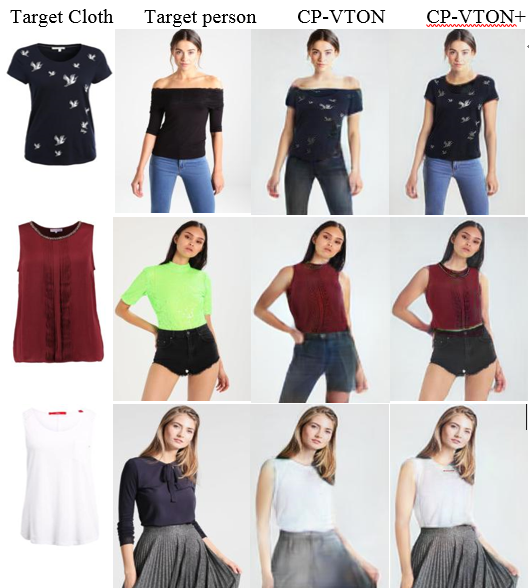
\includegraphics[height=6.5cm, scale=1]{figures/cpvton_cpvton+keyresult.png}   % TODO
\caption{The proposed VTON results}
\label{fig:cpvton_cpvton+keyresult}
\end{figure}

The contributions of this work are three-fold. First, we provide the classified performance evaluations of existing Image-based algorithms. Second, the origins are the limitations and reason of seemingly well working of the existing algorithms are  identified. Finally, a new pipeline is proposed to tackles the identified problems. The proposed pipeline not simply solves the identified problems but it also demonstrate the level of effects of them.
